\let\negmedspace\undefined
\let\negthickspace\undefined
\documentclass[journal]{IEEEtran}
\usepackage[a5paper, margin=10mm, onecolumn]{geometry}
%\usepackage{lmodern} % Ensure lmodern is loaded for pdflatex
\usepackage{tfrupee} % Include tfrupee package

\setlength{\headheight}{1cm} % Set the height of the header box
\setlength{\headsep}{0mm}     % Set the distance between the header box and the top of the text

\usepackage{gvv-book}
\usepackage{gvv}
\usepackage{cite}
\usepackage{amsmath,amssymb,amsfonts,amsthm}
\usepackage{algorithmic}
\usepackage{graphicx}
\usepackage{textcomp}
\usepackage{xcolor}
\usepackage{txfonts}
\usepackage{listings}
\usepackage{enumitem}
\usepackage{mathtools}
\usepackage{gensymb}
\usepackage{comment}
\usepackage[breaklinks=true]{hyperref}
\usepackage{tkz-euclide} 
\usepackage{listings}
% \usepackage{gvv}                                        
\def\inputGnumericTable{}                                 
\usepackage[latin1]{inputenc}                                
\usepackage{color}                                            
\usepackage{array}                                            
\usepackage{longtable}                                       
\usepackage{calc}                                             
\usepackage{multirow}                                         
\usepackage{hhline}                                           
\usepackage{ifthen}                                           
\usepackage{lscape}
\begin{document}
\bibliographystyle{IEEEtran}
\title{1.8.19}
\author{EE25BTECH11002 - Achat Parth Kalpesh }
{\let\newpage\relax\maketitle}
\renewcommand{\thefigure}{\theenumi}
\renewcommand{\thetable}{\theenumi}
\setlength{\intextsep}{10pt} % Space between text and floats
\numberwithin{equation}{enumi}
\numberwithin{figure}{enumi}
\renewcommand{\thetable}{\theenumi}
\parindent 0px


\textbf{Question:}\\
If $\vec{Q}$\brak{0, 1} is equidistant from $\vec{P}$\brak{5, -3} and $\vec{R}$\brak{x, 6}, find the values of x. Also find the distances $\vec{QR}$ and $\vec{PR}$.\\

\textbf{Solution:}\\
Let the given points be represented by the column vectors $\vec{P}$, $\vec{Q}$, and $\vec{R}$.
\begin{align}
    \vec{P} = \myvec{5 \\ -3}, \quad \vec{Q} = \myvec{0 \\ 1}, \quad \vec{R} = \myvec{x \\ 6}
\end{align}
According to given condition;
\begin{align}
\norm{\vec{P} - \vec{Q}}^2 = \norm{\vec{R} - \vec{Q}}^2
\end{align}
The squared norm of a vector $\vec{v}$ is given by the matrix product $\vec{v}^\top\vec{v}$.
\begin{align}
\brak{\vec{P} - \vec{Q}}^\top \brak{\vec{P} - \vec{Q}} = \brak{\vec{R} - \vec{Q}}^\top \brak{\vec{R} - \vec{Q}} \label{eq:0.3}
\end{align}

\begin{align}
\brak{\vec{P}^{\top} - \vec{Q}^{\top}} \brak{\vec{P} - \vec{Q}} &= \brak{\vec{R}^{\top} - \vec{Q}^{\top}} \brak{\vec{R} - \vec{Q}}\\
\vec{P}^{\top}\vec{P} - 2\vec{Q}^{\top}\vec{P} &= \vec{R}^{\top} \vec{R} - 2\vec{R}^{\top}\vec{Q}\\
\myvec{5 & -3}\myvec{5 \\ -3} - 2\myvec{0 & 1}\myvec{5 \\ -3} &= \myvec{x & 6}\myvec{x \\ 6} - 2\myvec{x & 6}\myvec{0 \\ 1}\\
\brak{5}\brak{5} + \brak{-3}\brak{-3} - 2\brak{0}\brak{5} -2\brak{1}\brak{-3} &= \brak{x}\brak{x} + \brak{6}\brak{6} -2\brak{x}\brak{0} - 2\brak{6}\brak{1} \\
25 + 9 + 6 &= x^2 + 36 -12 \\
x^2 &= 16 \\
    \implies x &= \pm 4
\end{align}

Therefore, the two possible vectors for $\vec{R}$ are:
\begin{align}
\vec{R}_1 &= \myvec{4 \\ 6}  \\  \vec{R}_2 &= \myvec{-4 \\ 6}
\end{align}


\begin{align}
     \norm{\vec{Q} - \vec{R}}&= \norm{\vec{P} - \vec{Q}} = \sqrt{5^2 + \brak{-4}^2} = \sqrt{41} \approx 6.40
\end{align}

\begin{itemize}
    \item For $\vec{R}_1$:
    \begin{align}
     \norm{\vec{R_1} - \vec{P}} &= \norm{ \myvec{4 - 5 \\ 6 - \brak{-3}}}  = \norm{ \myvec{-1 \\ 9}} \\
    &= \sqrt{\brak{-1}^2 + 9^2} = \sqrt{82} \approx 9.06
    \end{align}
    \item For $\vec{R}_2$:
    \begin{align}
    \norm{\vec{R}_2 - \vec{P}} &= \norm{\myvec{-4 - 5 \\ 6 - \brak{-3}}}  = \norm{\myvec{-9 \\ 9}} \\
    &= \sqrt{\brak{-9}^2 + 9^2} = \sqrt{162} = 9\sqrt{2} \approx 12.73
    \end{align}
\end{itemize}

\begin{figure}[h!]
    \centering
    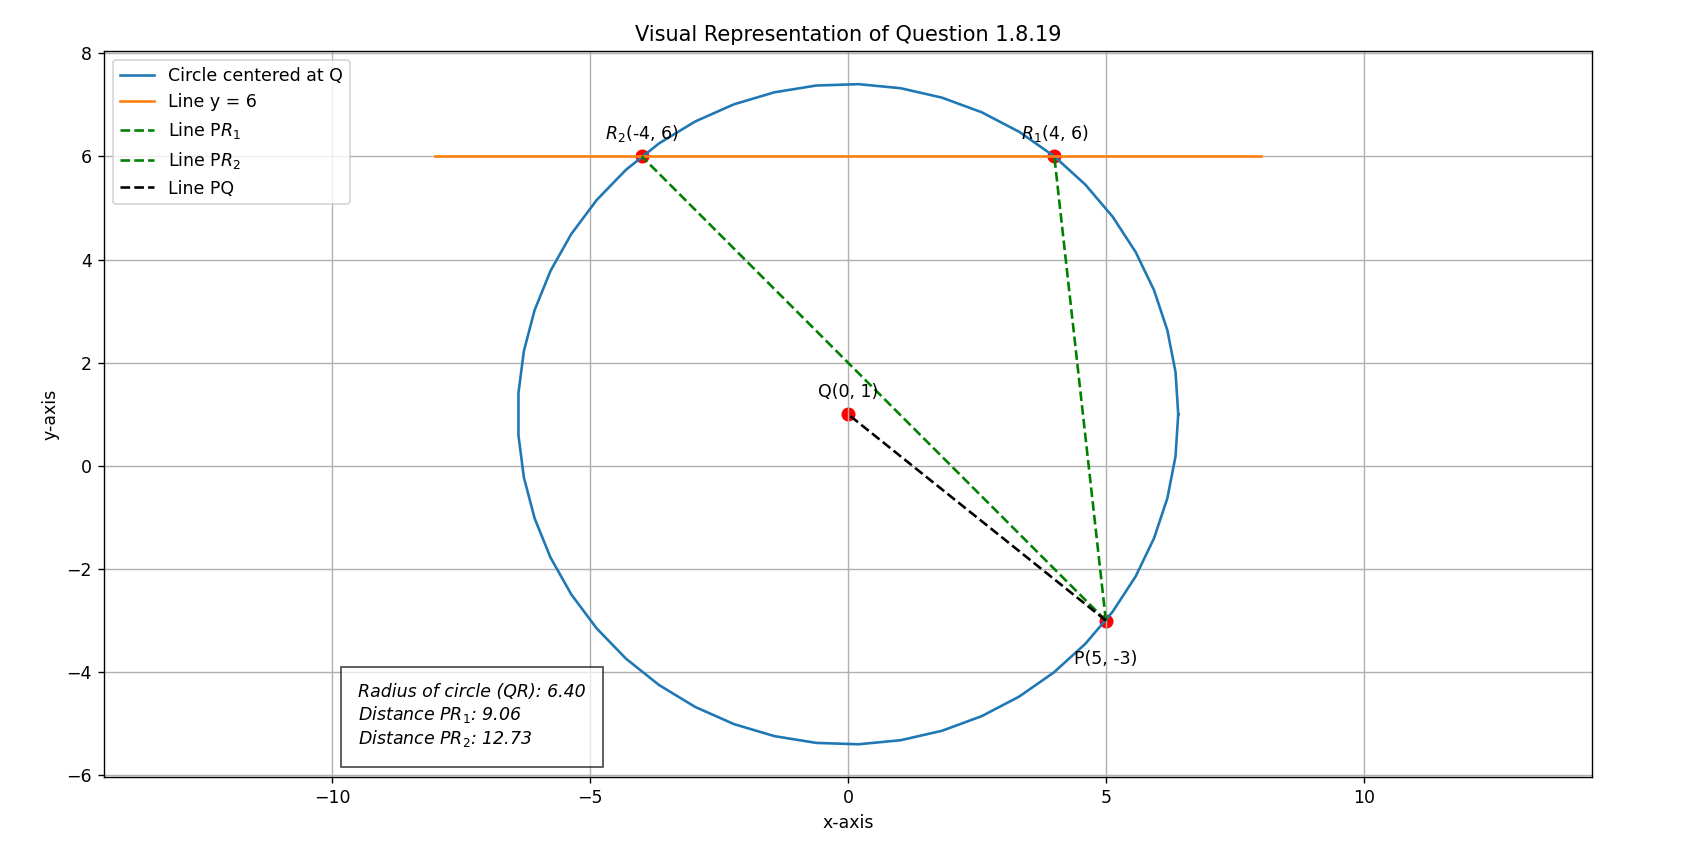
\includegraphics[width=0.9\columnwidth]{figs/pure_python.png}
    \caption{Visual representation of the solution. The points $R_1$ and $R_2$ are the intersections of the circle centered at Q and the line $y=6$.}
    \label{fig:fig}
 \end{figure}

\end{document}